% *********************************************************************
% © 2010–2022 Jeremy Sylvestre
%
% Permission is granted to copy, distribute and/or modify this document
% under the terms of the GNU Free Documentation License, Version 1.3 or
% any later version published by the Free Software Foundation; with no
% Invariant Sections, no Front-Cover Texts, and no Back-Cover Texts. A
% copy of the license is included in the appendix entitled “GNU Free
% Documentation License” that appears in the output document of this
% PreTeXt source code. All trademarks™ are the registered® marks of
% their respective owners.
%
% *********************************************************************

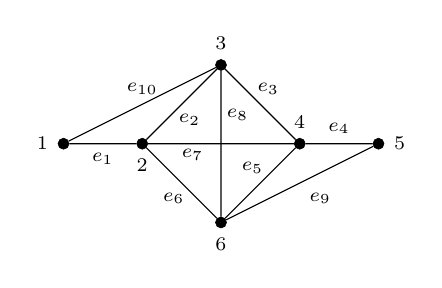
\begin{tikzpicture}[
	vertex/.style={ circle, draw, very thin, fill, inner sep=0pt, minimum size=4pt },
	vertexg/.style={ black!40!white, circle, draw, very thin, fill, inner sep=0pt, minimum size=4pt },
	vertexo/.style={ circle, draw, very thin, inner sep=0pt, minimum size=4pt }
]

\node at (0,0) (one) [vertex,label=left:$\scriptstyle 1$] {};
\node at (1,0) (two) [vertex,label=below:$\scriptstyle 2$] {};
\node at (2,1) (three) [vertex,label=above:$\scriptstyle 3$] {};
\node at (3,0) (four) [vertex,label=above:$\scriptstyle 4$] {};
\node at (4,0) (five) [vertex,label=right:$\scriptstyle 5$] {};
\node at (2,-1) (six) [vertex,label=below:$\scriptstyle 6$] {};
\draw (one) to node[below] {$\scriptstyle e_1$} (two)
  to node[below,xshift=0.1cm,y=-0.1cm] {$\scriptstyle e_2$} (three)
  to node[above,xshift=0.1cm] {$\scriptstyle e_3$} (four)
  to node[above] {$\scriptstyle e_4$} (five);
\draw (four) to node[above,xshift=-0.1cm] {$\scriptstyle e_5$} (six)
  to node[below,xshift=-0.1cm] {$\scriptstyle e_6$} (two)
  to node[below,near start,xshift=0.1cm,yshift=0.05cm] {$\scriptstyle e_7$} (four);
\draw (three) to node[right,near start,xshift=-0.05cm,yshift=-0.1cm] {$\scriptstyle e_8$} (six)
  to node[below right] {$\scriptstyle e_9$} (five);
\draw (one) to node[above] {$\scriptstyle e_{10}$} (three);

\end{tikzpicture}
